\documentclass[10 pt]{beamer}
\usetheme{Madrid}
\usepackage[utf8]{inputenc}
\usepackage{xspace}
\usepackage{graphicx,graphics} 
\usepackage{color}
\usepackage{amsmath}
\usepackage{amsfonts}
\usepackage{amssymb}
\usepackage{amsthm}
\usepackage{algorithm}
\usepackage{algorithmic}
\usepackage{longtable}
\usepackage{complexity}
\usepackage{tkz-graph}
\usepackage{float}
\usepackage{multicol}
\usepackage{setspace}
\usepackage[absolute,overlay]{textpos}
\graphicspath{{fig/}}

\tikzset{
  LabelStyle/.style = { rectangle, rounded corners, draw,
                       font = \bfseries },
  EdgeStyle/.append style = {-} }
\title{Deterministic Scheduling of Periodic Messages for Cloud RAN}

\author{{\bf Maël~Guiraud}}


\institute[Nokia Bell Labs, DAVID-UVSQ] 
{
  DAVID, Universit\'e de Versailles Saint Quentin -
  Nokia Bell Labs France \\
}

\subject{Theoretical Computer Science}

\begin{document}


\begin{frame}

  \titlepage
  \centering
  
\includegraphics [width=15mm]{logod.png} \hspace{1cm} 
\includegraphics [width=20mm]{logon.png} \hspace{1cm} 
\includegraphics [width=20mm]{logo.png} \\
\end{frame}




\begin{section}{Introduction}

\begin{frame}{Context}
  \centering
    A Base Transceiver Station
  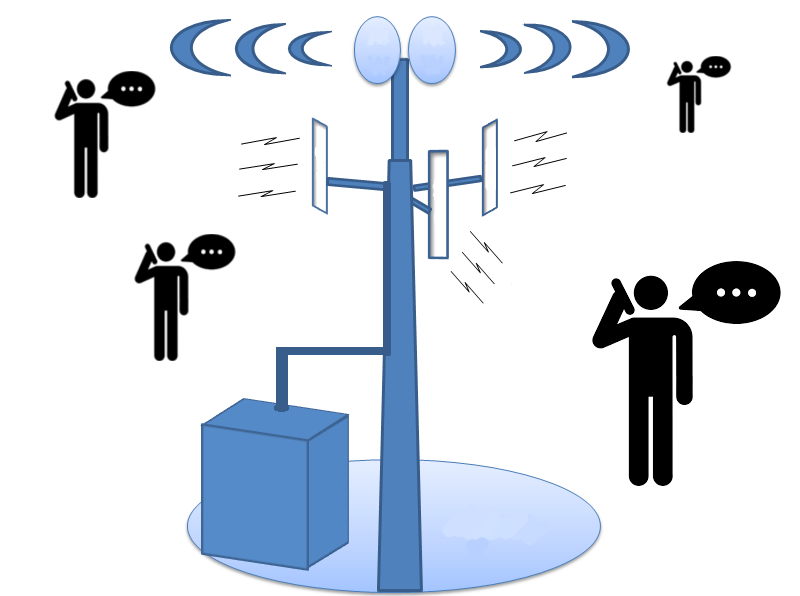
\includegraphics[scale=0.3]{btsppl.png}

\end{frame}


\begin{frame}{Context}
  \centering
  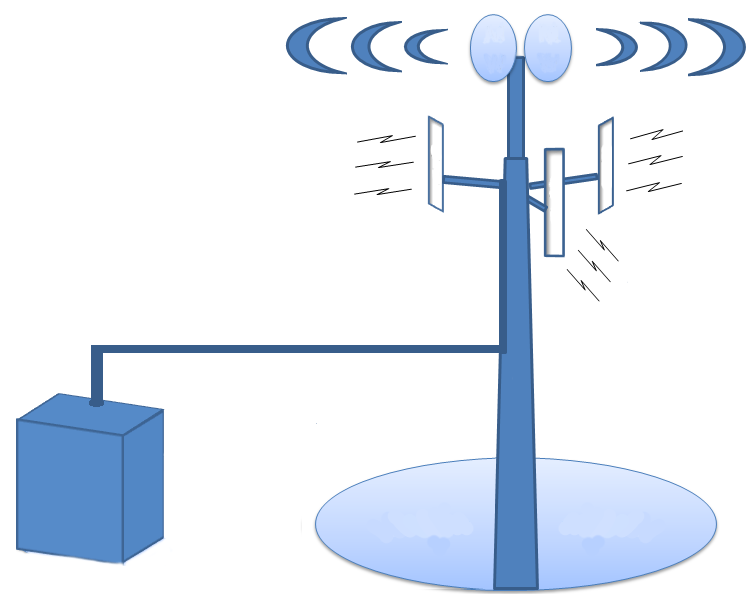
\includegraphics[scale=0.2]{cloudbts.png}\\
  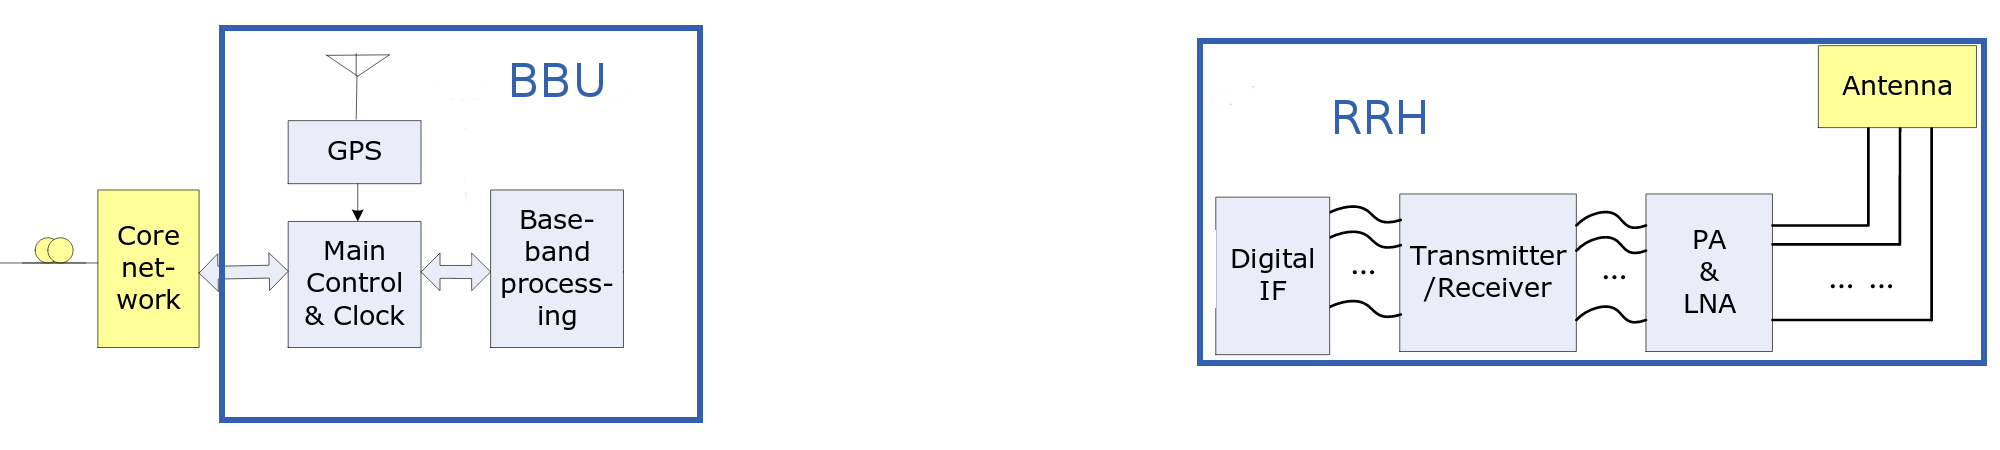
\includegraphics[scale=0.175]{BBURRH.png}
\end{frame}



\begin{frame}{Context}
  \centering
  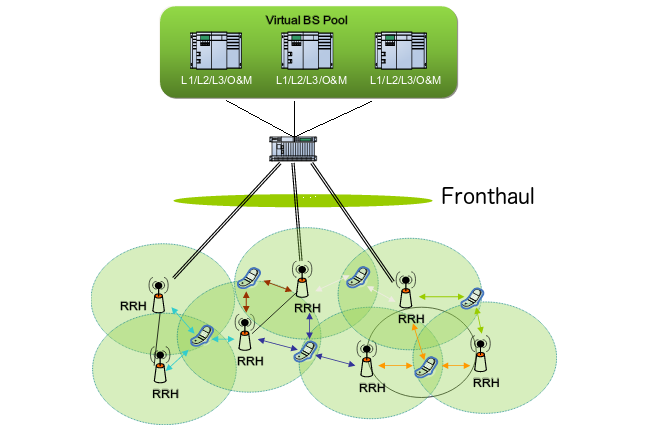
\includegraphics[scale=0.5]{CRAN}\\
  
\end{frame}

\begin{frame}{Problematic}
  \centering
  
  
 \begin{multicols}{2}
Specificity of Fronthaul network :
\vspace{1cm}
\begin{itemize}
\item Highly loaded
\item Periodic traffic
\item \textcolor{red}{Latency must be guaranteed}
\end{itemize}
\vspace{0.5cm}
Current approaches: \begin{itemize}
\vspace{1cm}
\item Point to Point connections $\rightarrow$ Too expensive
\item Statistical multiplexing $\rightarrow$ No latency guarantee
\end{itemize}
\end{multicols}

\end{frame}

\end{section}

\begin{section}{Model, Problem}

\begin{subsection}{Network Modeling}

\begin{frame}{Model}

Dessin papier a faire.
Network vers graph associé
\begin{itemize}
\item Network $\rightarrow$ Weighted DAG
\item  Physical Delay of a link $\rightarrow$ Weight of the arc
\end{itemize}

 \end{frame}
 
 
 
 \begin{frame}{The communication process}
 
 The time is discretized.

Two parameters
\begin{itemize}
\item The period $P$
\item The size of a message $\tau$
\end{itemize}
\vspace{0.5cm}

Every $P$ units of time, a message of size $\tau$ is emitted from each RRH.

\vspace{0.5cm}
\begin{center}
  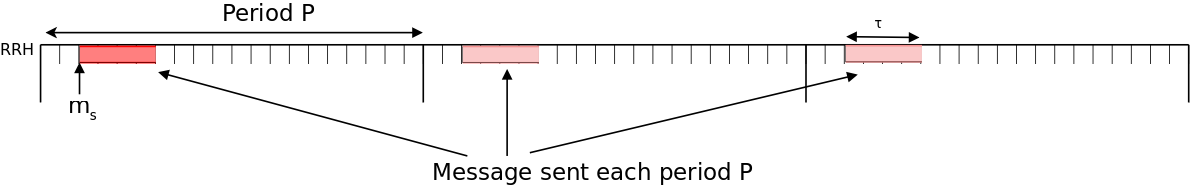
\includegraphics [width=11.5cm]{rrh} 
  \end{center}
 \vspace{0.5cm}
   
   The process is \textcolor{red}{periodic} : the message is emitted in each period at the same time, called \textcolor{blue}{offset}.
   
\end{frame}


 \begin{frame}{Collisions}

\begin{center}
\scalebox{0.4}{

\begin{tikzpicture}
  \SetGraphUnit{5}
    \tikzset{
  EdgeStyle/.append style = {->} }
   \tikzstyle{VertexStyle}=[shape = circle, draw, minimum size = 30pt]
   \renewcommand{\VertexLightFillColor}{orange}
  \Vertex[x=0,y=0, L = {\huge $a_3$}]{a3};
  \Vertex[x=0,y=4, L = {\huge $a_2$}]{a2}
  \Vertex[x=0,y=8, L = {\huge $a_1$}]{a1}


  \Vertex[x=16,y=4, L = {\huge $c$}]{c}
  
 \SetVertexNoLabel
  \Vertex[x=4,y=2]{n1}
  \Vertex[x=4,y=6]{n2}  
  \Vertex[x=12,y=3]{n4}
  \Vertex[x=8,y=3]{n6}
  \Vertex[x=8,y=5]{n7}
  \Vertex[x=10,y=6]{n8}



  \Edge(n1)(n2)
  \Edge(n8)(n4)
  \Edge(n8)(c)
  \Edge(n2)(n8)
  \Edge(n7)(n4)
  \Edge(n1)(n6)
  \Edge(n6)(n4)
  \Edge(a2)(n2)
  \Edge(n4)(c)

    
  \tikzset{
  EdgeStyle/.append style = {blue} }
  \Edge[label = 2](a1)(n2)   
   \Edge[label = 3](n2)(n7)
  
    \tikzset{
  EdgeStyle/.append style = {red} }
    \Edge[label = 2](a3)(n1)
      \Edge[label = 1](n1)(n7)
      
       \node (0) at (9,4){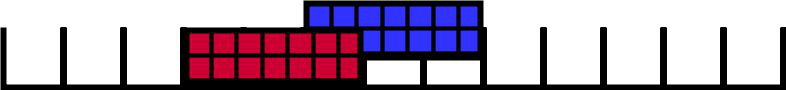
\includegraphics[scale=0.2]{col1.png}};


\end{tikzpicture}
}
\end{center}
\vspace{1cm}
\centering
There is a \textcolor{blue}{collision} between two routes when their messages go through the first vertex of a common arc at the same time.
\vspace{0.5cm}

 \textcolor{red}{Periodicity must be taken into consideration} 
\end{frame}

 \begin{frame}{Assignment }

\begin{center}
\scalebox{0.4}{

\begin{tikzpicture}
  \SetGraphUnit{5}
    \tikzset{
  EdgeStyle/.append style = {->} }
   \tikzstyle{VertexStyle}=[shape = circle, draw, minimum size = 30pt]
   \renewcommand{\VertexLightFillColor}{orange}
  \Vertex[x=0,y=0, L = {\huge $a_3$}]{a3};
  \Vertex[x=0,y=4, L = {\huge $a_2$}]{a2}
  \Vertex[x=0,y=8, L = {\huge $a_1$}]{a1}


  \Vertex[x=16,y=4, L = {\huge $c$}]{c}
  
 \SetVertexNoLabel
  \Vertex[x=4,y=2]{n1}
  \Vertex[x=4,y=6]{n2}  
  \Vertex[x=12,y=3]{n4}
  \Vertex[x=8,y=3]{n6}
  \Vertex[x=8,y=5]{n7}
  \Vertex[x=10,y=6]{n8}



  \Edge(n1)(n2)
  \Edge(n8)(n4)
  \Edge(n8)(c)
  \Edge(n2)(n8)
  \Edge(n7)(n4)
  \Edge(n1)(n6)
  \Edge(n6)(n4)
  \Edge(a2)(n2)
  \Edge(n4)(c)

    
  \tikzset{
  EdgeStyle/.append style = {blue} }
  \Edge[label = 2](a1)(n2)   
   \Edge[label = 3](n2)(n7)
  
    \tikzset{
  EdgeStyle/.append style = {red} }
    \Edge[label = 2](a3)(n1)
      \Edge[label = 1](n1)(n7)
      
       \node (0) at (9,4){
\includegraphics[scale=0.2]{col2.png}};


\end{tikzpicture}
}
\end{center}
\vspace{1cm}
\centering
Choosing the offset such that there are no collisions.
\vspace{0.5cm}

An \textcolor{blue}{assignment} is a choice of offsets for each route without collisions.
\end{frame}
\end{subsection}



\begin{subsection}{Problem PALL}
\begin{frame}{Full process}
In each BBU, one can choose the \textcolor{blue}{waiting time} before sending back the answer.\\

\begin{center}
  \includegraphics[scale=0.7]{BBU}\\
 \end{center} 

\textbf{Problem:}

Given a routed network, a period and a message size, find an assignment such that there is no collisions.
\end {frame}
\begin{frame}
Two measures to optimize.
 \begin{multicols}{2}
PALL:
\begin{itemize}
\item The RRH send their message at different dates in the period.
\item Local latency constraint.
\item Minimizing the process time on the longest route.
\end{itemize}
\vspace{0.5cm}
SPALL:
\begin{itemize}
\item The RRH send their message at the same date (Synchronized).
\item Global time constraint.
\item Minimizing the time between the emission of the first message and the reception of the last message.
\end{itemize}
\end{multicols}

The optimal solutions for PALL and SPALL are not the same.
\end{frame}
\end{subsection}


\end{section}

\begin{section}{Results on a common topology}

\begin{subsection}{A star routed Network}
\begin{frame}{Different topologies}

The  {\bf conflict depth} of a route is defined as the number of first arcs shared with other routes.

The conflict depth of a routed network is the maximal conflict depth of the routes in the network.
  \centering
   \begin{multicols}{2}


\scalebox{0.25}{
\begin{tikzpicture}
    \SetGraphUnit{5}
  \tikzstyle{VertexStyle}=[shape = circle, draw, minimum size = 50pt]
  \Vertex[x=0,y=0]{a3}
  \Vertex[x=0,y=4]{a2}
  \Vertex[x=0,y=8]{a1}
  
  \Vertex[x=16,y=0]{c3}
  \Vertex[x=16,y=4]{c2}
  \Vertex[x=16,y=8]{c1}
  
  \SetVertexNoLabel
  \Vertex[x=4,y=4]{SL}
  \Vertex[x=12,y=4]{SS}  
  \tikzset{
  EdgeStyle/.append style = {<-,green} }
  \Edge(c1)(SS)
  \Edge(SL)(a1)
  
  \tikzset{
  EdgeStyle/.append style = {blue} }
  \Edge(c2)(SS)
  \Edge(SL)(a2)
  
  \tikzset{
  EdgeStyle/.append style = {red} }
  \Edge(c3)(SS)
  \Edge(SL)(a3)
  
  \tikzset{
  EdgeStyle/.append style = {black} }
  \Edge(SS)(SL)
  


\end{tikzpicture}
}

 \vspace{1cm}
\centering
 Conflict depth one.
 

 

 
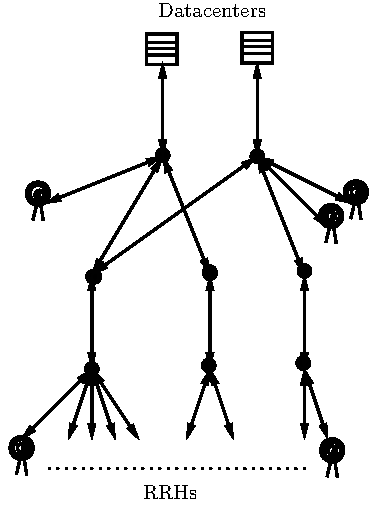
\includegraphics[scale=0.5]{extendendgraphgrey}\\
 \centering

 Conflict depth two.

\end{multicols}
\end{frame}

\begin{frame}{NP-Hardness}
   \begin{multicols}{2}
   PALL:
   \begin{itemize}
   \item Hard on conflict depth $2$: reduction from k-coloring problem
   \item Hard on conflict depth $1$ if the shared arc is not bidirectional.
   \end{itemize}
   
   SPALL:
   \begin{itemize}
    \item Hard on conflict depth $2$ 
       \item Hard on conflict depth $1$: reduction from two processors scheduling problem.
   \end{itemize}
   \end{multicols}

\end{frame}
\end{subsection}


\begin{subsection}{Results}

  \begin{frame}{Performances of the algorithms}
\centering
  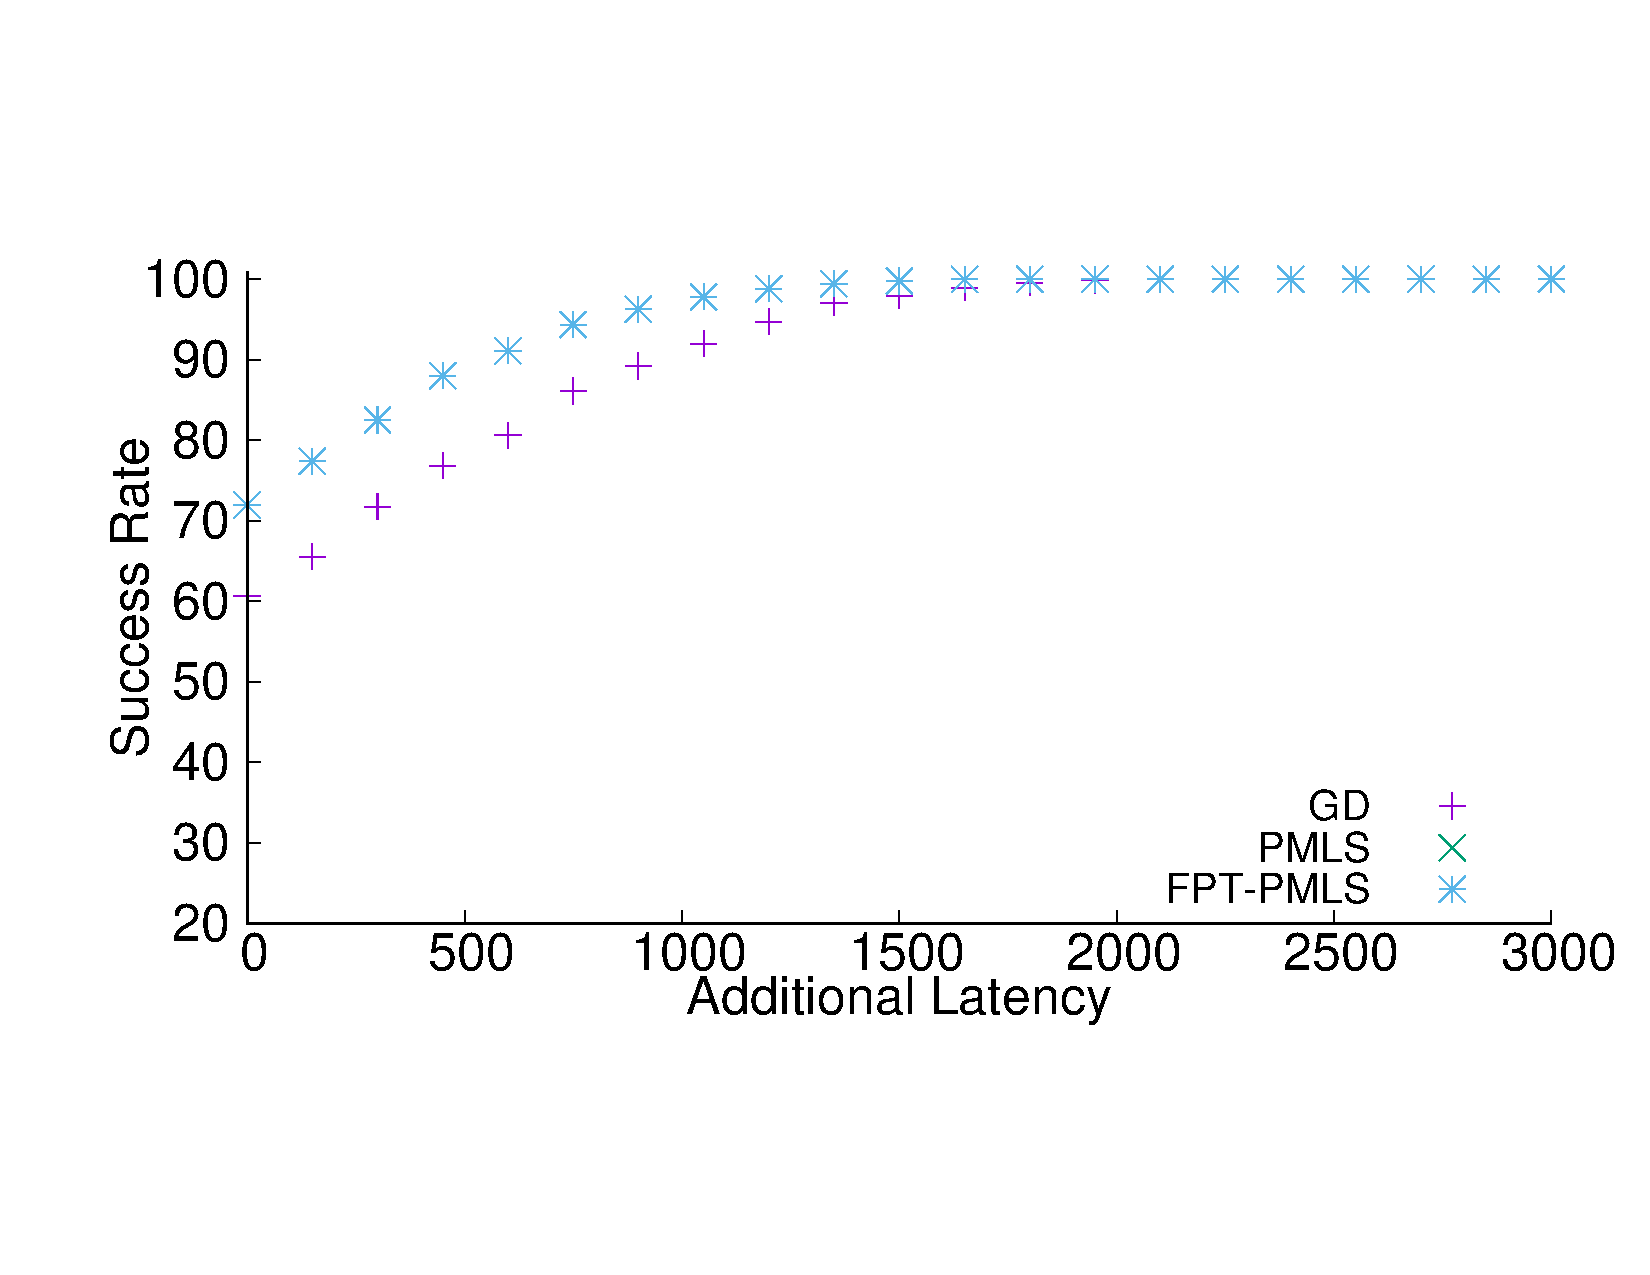
\includegraphics[scale=0.4]{retour_21000.pdf}\\
  
    Period : $20.000$ tics -  Load : $95\%$
  \end{frame}
  
    \begin{frame}{Deterministic vs Stochastic}
\centering
\vspace{-2cm}
  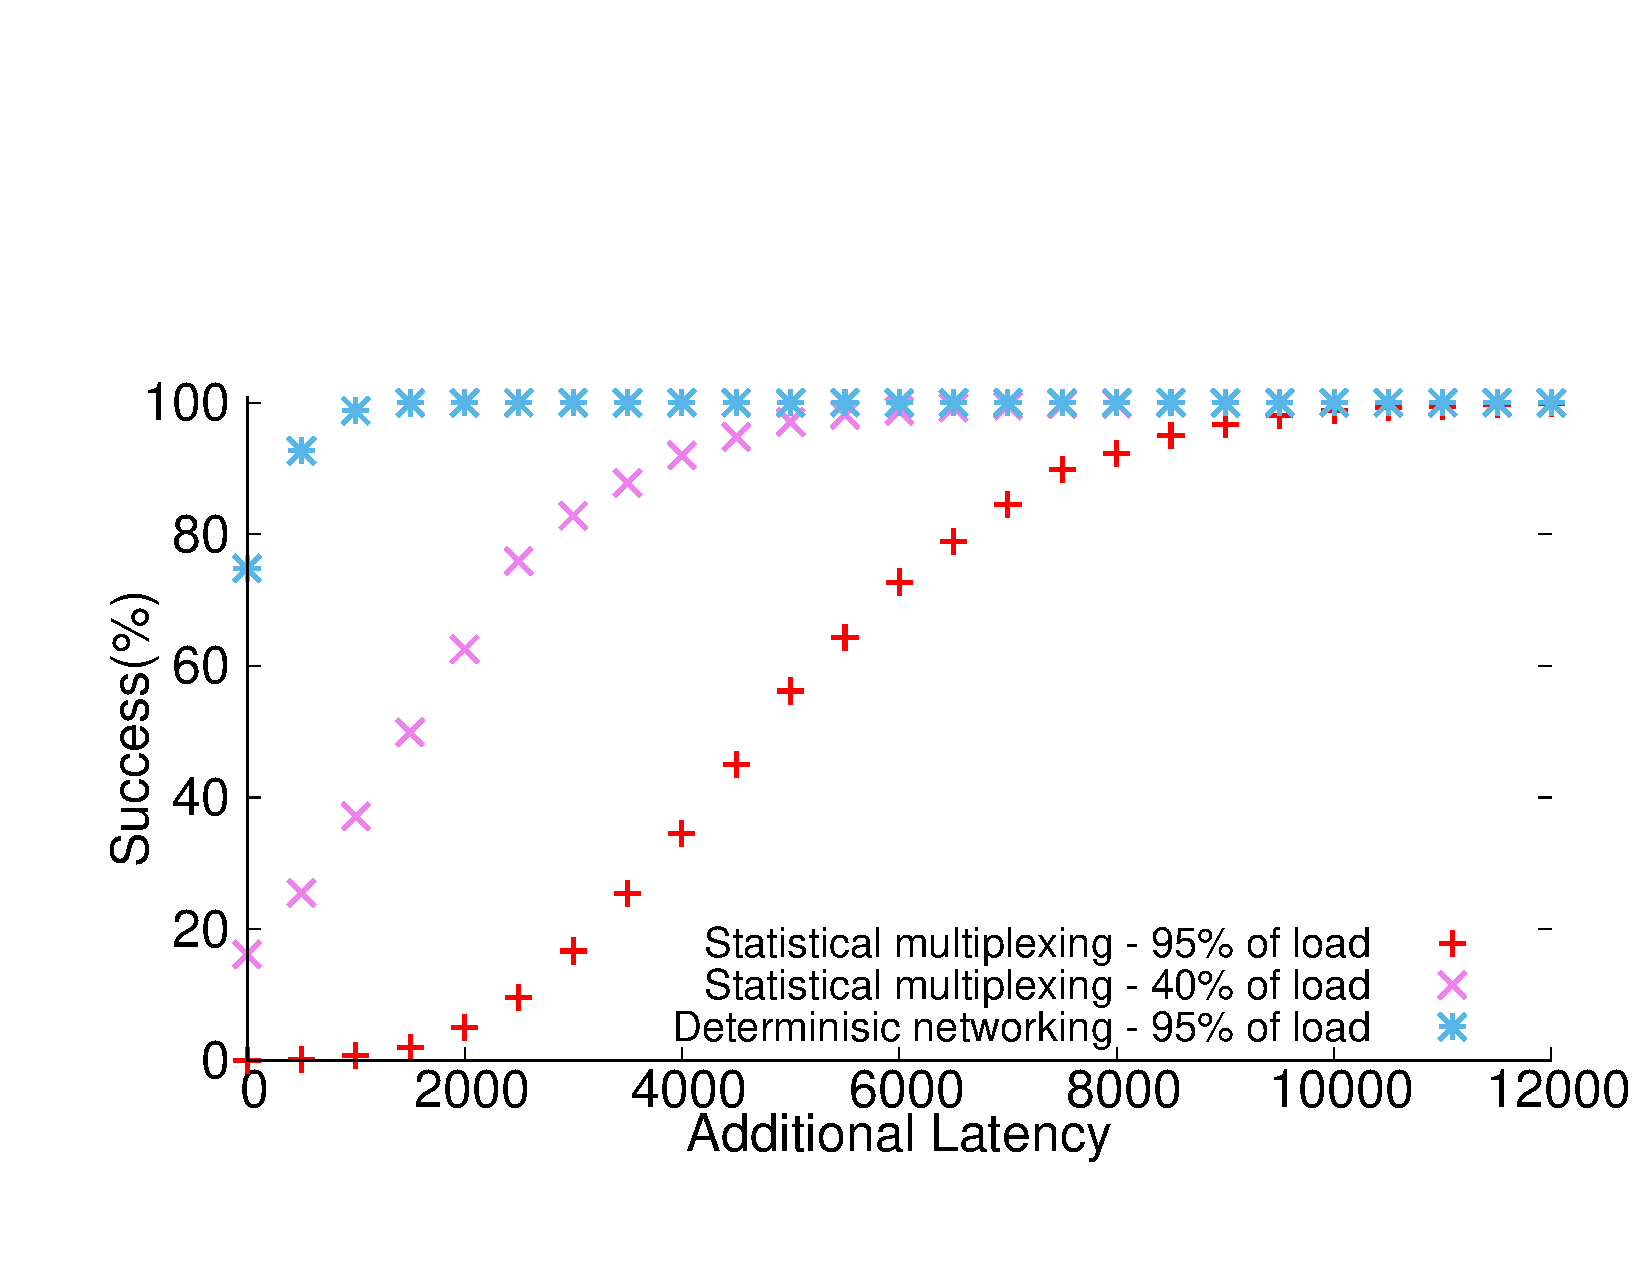
\includegraphics[scale=0.4]{stochastic.pdf}\\
  
  Period : $20.000$ tics - Load : $95\%$
  \end{frame}
  
  

\end{subsection}


\end{section}


\begin{section}{Technical intergration}

  \begin{frame}{TSN}
Parler de l'intergration avec TSN
  

\end{frame}

\end{section}




\end{document}
